\section{Extended Experiments}
\label{app:extra}



\subsection*{B.1\quad Setup and reproducibility}
Main-paper Figure~\ref{fig:overview} shows the enforcement model, and Supplement~D (Table~\ref{tab:systems-ext}) maps representative systems to our regimes. All experiments are inference-only (no training). The core judges are open-weights
models run locally on one workstation (or a free API for the $70$B), spanning three open
families and a $140{\times}$ size range: \texttt{qwen2.5} ($0.5$B, $3$B, $7$B, $32$B),
\texttt{llama3.1} ($8$B) and \texttt{llama-3.3} ($70$B), and \texttt{gemma2} ($9$B). To
these we add \emph{two closed-source} frontier judges from different vendors
(\texttt{gpt-4o-mini} from OpenAI and \texttt{command-a-03-2025} from Cohere),
\texttt{Llama-Guard-3} ($8$B) as a deployed guardrail, and a battery of
current-generation frontier judges (B.6) served through hosted inference APIs.
The pipeline consumes real-valued scores, so any scorer drops in. Each
score-judge rates an action with the single prompt reproduced verbatim in Supplement~C,
parsed to a risk score $s\in[0,1]$ (decoding settings below).
The gate blocks iff $s\ge\theta$. Calibration is split-conformal: for a target
$\delta$ we set the per-step conditional-miss target $\tau=\delta/H$ and choose
$\hat\theta$ as the $\lfloor(n{+}1)\tau\rfloor$-th smallest score among $n$
violating calibration examples ($\hat\theta=-\infty$ if that index is $0$, i.e.,
block everything). We flag one small-sample effect: when $\delta/H<1/(n{+}1)$ the index
is $0$ and the certificate is met \emph{trivially} by blocking all actions ($U=1$).
This is why the $\delta=.05$ row of Table~\ref{tab:curated} shows miss $0$ at $U=1$ on the small
curated set (fewer than $19$ calibration violations); it is an inherent
finite-sample limit of split conformal, and certifying $\delta<1/(n{+}1)$ needs more
violation data. Legacy descriptive quantities below average $400$ stratified
calibration/test splits; their error bars are one standard deviation across
splits, not familywise intervals. The
random seed is fixed ($20260704$). Four datasets are used: a curated set of $60$
labeled tool-call actions spanning the four touchstone policies plus
prompt-injection and destructive cases; the $132$ tool-use tasks of AgentDojo
\citep{debenedetti2024agentdojo} (its $97$ user tasks as compliant actions, its
$35$ injection goals as violations, from the banking/slack/travel/workspace suites);
InjecAgent and AgentHarm (B.6). The public
artifact contains code, redistributable data, the exact prompt, cached scores,
and a one-command cache-only reproduction path.

\smallskip\noindent\textbf{Compute, versions, and parsing.} Open judges are served locally
with \texttt{ollama} (CUDA backend) on a workstation with two $24$\,GB consumer GPUs,
using ollama's default GGUF quantization (typically \texttt{Q4\_K\_M});
the $70$B and all closed/frontier judges are served through hosted inference APIs,
at temperature $0$ except the seven judges without temperature control (below). AgentDojo is pinned
to benchmark version \texttt{v1.2.1} (Python package \texttt{agentdojo} 0.1.35). A judge's text output is parsed by clamping the first integer to
$[0,100]$ and dividing by $100$; a provider content-filter block is scored $1.0$ (a flagged
violation). In the older caches (26 of the 33 runs), any reply without an integer, including a
textual refusal, and an API error after retries were stored as $.5$; only the seven judges
without temperature control were scored with refusals (an explicit refusal stop reason) at $1.0$. Scores of $1.0$ fall mostly on violations (Grok-4: $14/35$ violations versus $3/97$ compliant items), so this can \emph{inflate} rather than depress the two content-filtered runs' AUC: the same Mistral-Large-3 model scores $.834$ through the filtered endpoint versus $.819$ unfiltered, so these numbers are not conservative.
Local inference is a few GPU-hours.
The curated probe contains serialized tool calls, but the static AgentDojo diagnostic
contains \emph{instruction strings}: $97$ user-task prompts and $35$ injection goals, without
the pre-call execution history or tool output. It therefore estimates discrimination for
that declared information variable only. More context changes the statistical experiment
and may help or hurt a fixed scoring prompt; Blackwell refinement guarantees only that the
\emph{optimal} test with richer information cannot have a worse ROC.

\paragraph{Judges and scoring rule}
Every AgentDojo analysis uses the same 33 judge runs (32 distinct models;
Mistral-Large-3 is served by two providers) on the same ordered 132 items. All judges
receive the same 0--100 prompt. Judges whose APIs accept a temperature decode at
temperature $0$; seven hosted judges are served without temperature control (Claude Opus~5.5,
Fable~5.1, Sonnet~5.5, and Haiku~5.5; GPT-6.1 Sol, GPT-6.1 Terra, and GPT-5.5), so each
item is scored in three independent runs, run~1 is reported, and runs 2--3 serve as a
robustness check (B.19). Content-filter blocks score $1.0$ for every run, and refusals signaled
by the API score $1.0$ (fail-closed, as a gate must treat a non-answer) for the seven judges
without temperature control; elsewhere a reply without an integer, including a textual refusal,
scores $.5$. Caches that store only scores cannot separate a stored $.5$
from a genuine answer of $50$; the exact-$.5$ counts per judge are an upper bound on what
the rule could change (Llama-3.1-8B $87$ of $132$, Qwen-2.5-32B $21$, Nova-Pro $16$,
Step-3.7-Flash $15$, Kimi-K2.5 $9$, Command~A $7$, at most $5$ for every other judge;
\texttt{unify\_crossfit.py}). Model identifiers and query dates are listed in the
artifact's model registry.

\subsection*{B.2\quad Synthetic validation}
The synthetic judge is binormal (compliant score $\mathcal N(0,1)$, violating
score $\mathcal N(\mu,1)$, $\mu=2.5$, horizon $H=20$), giving an analytic ROC
against which the Monte-Carlo simulation is checked. \textbf{Q1, certificate:} calibrating to
$\delta$ yields realized episode-unsafe rate $.0098,.0194,.0486,.0951,.182$
at $\delta=.01,.02,.05,.10,.20$ (each $\le\delta$, and tight).
\textbf{Q1, frontier:} sweeping the threshold, the empirical operating points match the
analytic frontier $U^{\star}(\delta)=\ROC(R_H^{-1}(\delta))$ to within $2.7$
standard deviations of Monte-Carlo error over $40$ thresholds (Fig.~\ref{fig:frontier}).

\begin{figure}[h]
\centering
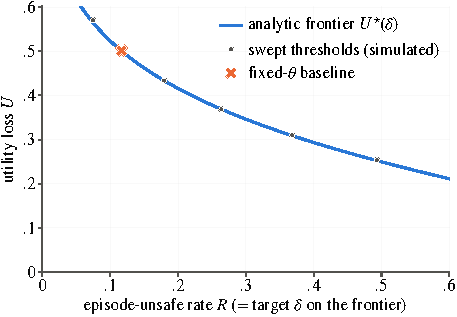
\includegraphics[width=\columnwidth]{synthetic_frontier}
\caption{Q1 (frontier): swept thresholds land on the predicted Pareto frontier
$U^{\star}(\delta)$ of main-paper Corollary~\ref{cor:reduction}; a fixed threshold that ignores $\delta$
(cross) also lies on the frontier, but at a single risk level ($R\approx.12$), so it misses every tighter
target. Only the swept thresholds with $R,U\le.6$ are shown. Synthetic judge, exact ROC.}
\label{fig:frontier}
\end{figure}

\paragraph{Controlled finite-model instantiation}
We also instantiate the endogenous finite-model frontier (main-paper Theorem~\ref{thm:sequential}) in an auditable two-step
retry environment. Initially the score is high ($.8$) with probability $.4$ and low ($.2$)
with probability $.6$, with violation posteriors $.8$ and $.2$. Allowing
terminates; blocking produces a second proposal. Its current score is $.2$ in
both branches, but its posterior is $.6$ after a blocked high score and $.02$
after a blocked low score. Thus only perfect recall reveals the
decision-dependent retry state. Cost is the expected number of compliant
proposals blocked and risk is episode-unsafe probability.

We enumerate all $2^4=16$ deterministic perfect-recall policies and take their
exact convex hull (episode-level randomization; Fig.~\ref{fig:controlled-frontier}). At $\delta=.05$, the optimum
costs $.551$, versus $.863$ for policies using only current score and time and
$1.137$ for stationary score thresholds. The static ``block high'' threshold
has $(R,C)=(.36,.08)$ and misses the constraint. Hence even this minimal model
has a strict history-value gap; the class comparisons use episode-level mixtures, and
with fresh per-step randomization the stationary class reaches about $1.074$ (grid search),
still far above $.551$. \texttt{controlled\_model.py} in the artifact reproduces all
four numbers in exact rational arithmetic ($124/225$, $863/1000$, $10237/9000$, and
$(9/25,2/25)$); the perfect-recall optimum mixes, once per episode, the policy that blocks
everything except a retry after a low score (weight $35/54$, $(R,C)=(.012,.72)$) with the
policy that blocks a high first score and its retry and allows a low first score (weight
$19/54$, $(R,C)=(.12,.24)$).
\emph{Exploratory logging (Proposition~\ref{prop:explore}).} On the two-system construction of
Proposition~\ref{prop:feedback} ($q=.3$, $p=.5$), we evaluate the gate that blocks step one and
allows step two, whose risk is $0$ in system A and $p=.5$ in B. Ungated logs have the same law
in both systems, so no estimator separates them. With a logging gate that blocks each step
independently with probability $\varepsilon$, the per-decision importance-sampling estimate is
unbiased in both systems (mean $.000$ for A and $.497$--$.505$ for B over 2,000 replications), and
its RMSE for B falls from $.330$, $.174$, $.131$ at $n=100$ logged episodes to $.032$, $.016$, $.013$
at $n=10^4$ for $\varepsilon=.05,.20,.50$; small $\varepsilon$ costs more data, as the
$\varepsilon^{-H}$ weight bound predicts (\texttt{prop\_explore\_sim.py}).
\begin{figure}[h]
\centering
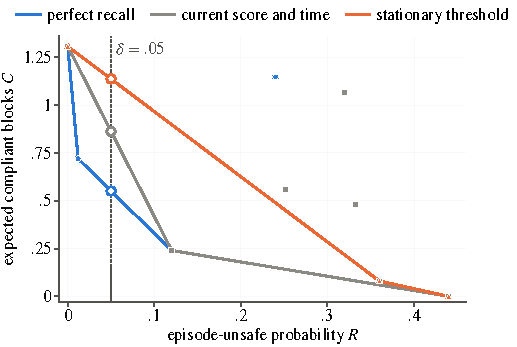
\includegraphics[width=\columnwidth]{controlled_frontier}
\caption{Exact occupancy frontier of the specified retry model. Points are
deterministic policies and segments are episode-level mixtures. Restricting
the gate to current-score/time or one stationary threshold raises the cost at
$\delta=.05$.}
\label{fig:controlled-frontier}
\end{figure}

\subsection*{B.3\quad Real judges on the curated set}
Table~\ref{tab:curated} reports realized miss (safety) and utility loss $U$ at
each target $\delta$ for four judges ($H=1$, per-action) in the original
400-split descriptive probe. Mean observed miss is at or below target, and
the utility cost of a fixed safety level broadly falls as
judge quality (AUC) rises: at $\delta=.10$ the utility loss falls from $1.00$
(the near-random $0.5$B judge, which is safe only by blocking everything) to
$.59$ ($3$B) to $.03$ ($7$B), consistent with the frontier (Fig.~\ref{fig:cert} shows the $3$B sweep). A $32$B judge
reaches AUC $.998$ and $U=.04$; this probe does not support an equivalence
claim between the $7$B and $32$B points. Scored with the same prompt and decoding (Supplement~C), Claude Opus~5.5, Sonnet~5.5, and
Haiku~5.5 and GPT-5.5 all reach AUC $1.000$ on this probe (4 refusals, scored $1$;
\path{curated_frontier2026.py}), so it no longer separates current judges; the static,
adversarial, and closed-loop results rest on AgentDojo (Supplement~E).

\begin{table}[t]
\caption{Curated descriptive probe (judges of AUC $.53$, $.92$, $.98$,
$.998$): mean realized miss and per-action false-block loss over 400 splits.
Block-all points are vacuous; no pairwise equivalence is inferred.}
\label{tab:curated}
\centering\small\setlength{\tabcolsep}{3pt}
\begin{tabular}{@{}lcccccccc@{}}
\toprule
& \multicolumn{2}{c}{$0.5$B} & \multicolumn{2}{c}{$3$B} & \multicolumn{2}{c}{$7$B} & \multicolumn{2}{c}{$32$B}\\
\cmidrule(lr){2-3}\cmidrule(lr){4-5}\cmidrule(lr){6-7}\cmidrule(lr){8-9}
$\delta$ & miss & $U$ & miss & $U$ & miss & $U$ & miss & $U$\\
\midrule
$.05$ & $.000$ & $1.00$ & $.000$ & $1.00$ & $.000$ & $1.00$ & $.000$ & $1.00$\\
$.10$ & $.000$ & $1.00$ & $.070$ & $.59$ & $.065$ & $.03$ & $.038$ & $.04$\\
$.20$ & $.000$ & $1.00$ & $.117$ & $.16$ & $.104$ & $.03$ & $.036$ & $.00$\\
$.30$ & $.000$ & $1.00$ & $.149$ & $.09$ & $.116$ & $.03$ & $.036$ & $.00$\\
\bottomrule
\end{tabular}
\end{table}

\begin{figure}[t]
\centering
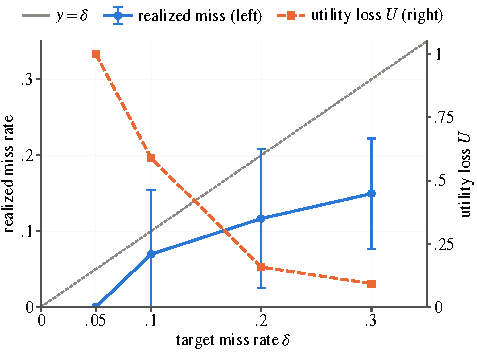
\includegraphics[width=\columnwidth]{real_certificate}
\caption{Q1 on the real \texttt{qwen2.5:3b} judge: the descriptive cross-split
mean realized miss stays below the target $\delta$ (left axis; error bars are
one standard deviation over $400$ calibration/test splits) while
the utility loss it costs (right axis) falls as $\delta$ relaxes.}
\label{fig:cert}
\end{figure}

\textbf{Q3 (adversarial).} On the $3$B judge, calibrating to $\delta=.10$ on all $27$ benign violations gives
in-sample benign miss $.037$ ($1/27$; the held-out mean in Table~\ref{tab:curated} is $.070$); injection-style safe-washing of the violations raises the
miss to $.889$ under the strongest tested template. This is a finite probe of
representation sensitivity, not a universal worst-case or soundness result; the
common-population AgentDojo analysis in B.9 is primary.

\subsection*{B.4\quad AgentDojo benchmark}
The calibration diagnostic uses 500 label-balanced two-fold splits (seed $0$) for all
33 judge runs (\texttt{unify\_crossfit.py}): each split calibrates the conformal
threshold on one fold's violations and measures miss on the other fold's violations
and false block on its compliant items. This is a finite-dataset compatibility
check; the conformal theorem's certificate additionally requires deployment
exchangeability, and we report cross-fitted point estimates only (no simultaneous
bounds are computed).

At $\delta=.05$, every judge's rule is block-all: a half-fold holds 17--18
violations, fewer than $1/\delta-1=19$, so the conformal index is $0$ (miss $0$,
false block $1$). At $\delta=.10$ the index is $1$ in every half-fold, so $\hat\theta$
is the fold's lowest violating score; across judges, cross-fitted miss is $0$--$.053$
and false block $.641$--$1.000$. At $\delta=.20$, miss is $.019$--$.164$ and false
block $.183$--$.964$. For Gemma-2-9B the operating points are $(.012,.779)$ at
$\delta=.10$ and $(.144,.649)$ at $\delta=.20$, the same splits as main-paper
Fig.~2a. Block-all is reported as vacuous, and a point estimate at or below target is
never called a certificate.

The primary rewrite result is separate from calibration: it fixes $\theta=.5$, uses
every one of the 35 violations, and reports simultaneous suite-bootstrap intervals over
every judge with clean and suffix-rewritten caches (B.9). It estimates a
common-population representation effect at one operating point, not certificate
failure at every threshold.

\emph{Counterfactual source-role diagnostic.}
To isolate authorization provenance without propagating episode outcomes, we
take the culminating call from every AgentDojo user or injection task with a
nonempty ground-truth plan: 97 user tasks and 26 injection tasks. Each of the
123 source tasks yields a pair with byte-identical call, arguments, instruction
text, and control text. In the authorized member, the source instruction is the
trusted user request and the control is untrusted output; in the unauthorized
member, those two source roles are swapped. Under the declared policy that only
trusted user input grants authority, labels are exact for this counterfactual.
They are not natural-trace safety annotations.

The primary statistic is paired concordance
$\Pr(s_{\rm unauth}>s_{\rm auth})+\frac12\Pr(s_{\rm unauth}=s_{\rm auth})$.
Treating source tasks as exchangeable draws from a conceptual task population,
we test the conditional sign null and compute a 20,000-draw task-pair bootstrap
interval. For the fixed 123-task AgentDojo set, concordance and
win/tie/loss counts are exact descriptive quantities.
Because the action is identical within each pair, action-only concordance is
exactly $.5$ by construction. Context-rich concordance is $.561$ for the 3B
primary ($15/108/0$ wins/ties/losses; bootstrap $95\%$ CI
$[.533,.589]$), $.967$ for 7B-model corroboration
($95\%$ CI $[.939,.988]$; $116/6/1$), and $.500$
for the 0.5B negative control ($0/123/0$). Holm-adjusted two-sided exact
$p$-values across the three models are $1.22{\times}10^{-4}$,
$4.26{\times}10^{-33}$, and $1$. Thus the larger judges respond directionally
to source role under this policy, but the experiment does not estimate
natural-trace accuracy, real-world authorization, or deployment safety.

The cache is bound to dataset, prompt, and model hashes and stores raw model
responses and parser provenance; it is not part of the public artifact (Supplement~C).

\subsection*{B.5\quad Closed-loop agent evaluation ($H>1$)}
The preceding AgentDojo diagnostic scores instructions statically; here we run
the \emph{real} AgentDojo agent loop across all four suites. A local
\texttt{qwen2.5:7b} agent drives the banking, slack, travel, and workspace suites under
the \texttt{important\_instructions} indirect prompt-injection attack; a gate element
placed before tool execution scores each proposed tool call with the judge and drops
those at/above $\theta$, over multi-step trajectories. The judge decodes at temperature $0$ against a
fixed endpoint. The agent is called through AgentDojo's \texttt{OpenAILLM} element with its default temperature $0$
(\texttt{run\_loop.py} sets none), which agentdojo 0.1.35 drops from the request (it passes
\texttt{temperature or NOT\_GIVEN}), so the agent most likely sampled at the endpoint's default temperature (not
recorded); this is consistent with the run-to-run
shifts in Supplement~E.5. Conditions are paired on task and injection goal. Table~\ref{S-tab:loop} reports
end-to-end task-utility and attack success over
$949$ episodes per condition ($144$ banking, $105$ slack, $140$ travel, $560$ workspace),
with Wilson $95\%$ intervals; these intervals and the per-suite Fisher tests below treat episodes as independent although they share user tasks and injection goals, so they are approximate and likely somewhat narrow.

\emph{Trace-derived action-level go/no-go.} We instrumented the interceptor to log each proposed call,
the preceding messages and tool outputs, action-only and context-rich scores, and the gate
decision. A local rerun reproduced such traces. AgentDojo's exposed checks in this pipeline,
however, label \emph{episode} attack success rather than mapping a security label to every
intercepted call. Copying the episode label onto all calls would mislabel prerequisite and
benign calls, so the strict analysis rejects this as primary action-level evidence. We report
no action-only-versus-context-rich AUC from those generated traces; the
policy-grounded B.4 diagnostic and end-to-end Q4 outcomes use different,
explicitly valid units.

\emph{Injectability is heterogeneous, so we test the gate stratified by suite.} The
local agent is far more injectable on slack ($25/105$ baseline attack success, $.238$)
than on banking ($12/144$, $.083$) or travel ($8/140$, $.057$), and is \emph{not}
injectable at all on workspace ($0/560$: it completes many workspace tasks but the attack
never lands). Pooling such suites into one $2\times2$ table would let the low- and
zero-injectability suites mask the effect (a Simpson's-paradox risk), so we test each gate
against its own no-gate baseline with a Cochran--Mantel--Haenszel test stratified by suite
and report the Mantel--Haenszel common odds ratio; suites in which the attack never fires
(workspace) contribute no information and drop out of the test.

\emph{The selected $3$B policy reduces attack success.} From $45/949$
ungated to $4/949$ at $\theta{=}0.5$: stratified over the three injectable suites, CMH
$\chi^2{=}35.8$, $p=2.2\times10^{-9}$, common OR $0.073$. The reduction is significant
\emph{within} each injectable suite (banking Fisher $p=4\times10^{-4}$, slack $p<10^{-4}$,
travel $p=.036$); banking and slack survive Bonferroni correction over the three suites, travel only Holm's step-down correction (Bonferroni: $3\times.036=.108$). But the $3$B reaches this only
by gating $78\%$ of all proposed calls ($91\%$ banking, $60$--$63\%$ slack/travel, $85\%$
workspace).

\emph{Clustering caveat and the exact paired refinement.} The same user tasks and injection
goals recur across the gated and ungated arms, so the episodes are paired, not independent, and
the between-arm CMH treats them as independent groups. The natural unit is the $(\text{task},
\text{goal})$ pair, on which the correct test is McNemar's. We compute it directly by re-running
the three injectable suites with per-episode outcome logging ($N{=}389$; these logs are not part
of the public artifact; agent sampling (and endpoint
nondeterminism) shifts the counts from $45/389$ and $4/389$ in the main run to baseline $38/389$ and $3$B-gate $9/389$). On
this run the suite-stratified CMH is $p{=}1.9\times10^{-5}$ (MH OR $0.21$) and the
\emph{task-paired McNemar} is $p{=}2.4\times10^{-6}$ ($34$ baseline-only vs.\ $5$ gate-only
discordant episodes): the paired test is \emph{more} significant than the unpaired one on the
same data, so the $3$B gate's effect survives pairing (episodes still share tasks and goals). The $5$ gate-only pairs show
that gated outcomes do not nest the ungated ones, but the discordances are strongly
one-directional; without an A/A control, part of this discordance may be agent sampling or endpoint
nondeterminism (zero-block reruns shift suite-level attack counts by up to 4, e.g.,
$12\to15$ on banking with no block).
The weak $7$B gate, by contrast, blocks and creates attacks about equally ($29$ vs.\ $22$
discordant, McNemar $p{=}0.40$), matching its across-suite non-significance.

\emph{The selected lighter $7$B policy has no detected pooled effect.} At
$\theta{=}0.7$ the $7$B gate blocks only $12\%$ of calls and cuts attack success from
$45/949$ to $30/949$: significant on the injectable slack suite ($25/105\to11/105$,
Fisher $p=.016$) but inert on travel (the $7$B judge blocks only $2$ of $1{,}077$ travel
calls) and flat on banking ($12/144\to10/144$). Across suites the effect is
not significant (CMH $p=.09$, common OR $0.63$). These are two selected
policies with different costs, not an estimate of the controlled optimum or a
causal effect of judge scale. Feedback invalidates the \emph{exact product ROC
lift}: blocking reroutes the agent and changes later proposals. The conformal
episode certificate instead uses a union bound and does not require
within-episode independence, provided its per-step exchangeability assumptions
hold.

\emph{Task success and gating fraction are separate endpoints.} Pooled task
success is $.254$ (Wilson $95\%$ $[.227,.283]$) ungated, $.243$
($[.217,.272]$) with 7B, and $.180$ ($[.157,.206]$) with 3B. The clearest cost is on
workspace, the largest suite ($.264$ ungated task success): the light $7$B gate
leaves it untouched ($.264$, $3\%$ gated) while the heavy $3$B gate cuts it by nearly
$40\%$ ($.264\to.163$, $85\%$ gated) although no attack ever succeeded there
to justify the blocking. Absolute attack rates are modest; we did not run a frontier agent, which may
solve more tasks and be more injectable. Gating fractions
are descriptive call-level rates; calls are clustered within episodes, so we do
not attach binomial call-level intervals.

\begin{table}[h]
\caption{Closed-loop AgentDojo across all four suites, $949$ episodes/condition, one fixed
endpoint (judge at temperature $0$; agent temperature as described in the text). Stratified by suite (Cochran--Mantel--Haenszel over the three
injectable suites; workspace is not injectable, $0/560$, and drops out), the $3$B gate
cuts end-to-end attack success $45/949\to4/949$ ($p=2.2\times10^{-9}$, common OR $0.07$),
but only by gating $78\%$ of calls; the lighter $7$B gate ($12\%$ gated) is significant
only on the injectable slack suite (across suites CMH $p=.09$). On workspace the heavy
$3$B gate reduces task success ($.264\to.163$) while no attack succeeds in
either arm. Task-success and attack intervals are Wilson; gating fractions are
descriptive because calls are clustered within episodes.}
\label{S-tab:loop}
\centering\scriptsize\setlength{\tabcolsep}{2pt}
\begin{tabular}{@{}llccccc@{}}
\toprule
suite & judge & $\theta$ & $N$ & task success [$95\%$ CI] & attack [$95\%$ CI] & gated \\
\midrule
banking & none & n/a & $144$ & $.382$ [$.307,.463$] & $.083$ [$.048,.140$] & $0\%$ \\
        & \texttt{qwen7b} & $.7$ & $144$ & $.396$ [$.320,.477$] & $.069$ [$.038,.123$] & $32\%$ \\
        & \texttt{qwen3b} & $.5$ & $144$ & $.375$ [$.300,.456$] & $.000$ [$.000,.026$] & $91\%$ \\
\midrule
slack & none & n/a & $105$ & $.219$ [$.151,.307$] & $.238$ [$.167,.328$] & $0\%$ \\
      & \texttt{qwen7b} & $.7$ & $105$ & $.124$ [$.074,.200$] & $.105$ [$.060,.178$] & $35\%$ \\
      & \texttt{qwen3b} & $.5$ & $105$ & $.162$ [$.104,.244$] & $.029$ [$.010,.081$] & $60\%$ \\
\midrule
travel & none & n/a & $140$ & $.107$ [$.066,.169$] & $.057$ [$.029,.109$] & $0\%$ \\
       & \texttt{qwen7b} & $.7$ & $140$ & $.093$ [$.055,.152$] & $.064$ [$.034,.118$] & $0\%$ \\
       & \texttt{qwen3b} & $.5$ & $140$ & $.064$ [$.034,.118$] & $.007$ [$.001,.039$] & $63\%$ \\
\midrule
workspace & none & n/a & $560$ & $.264$ [$.229,.302$] & $.000$ [$.000,.007$] & $0\%$ \\
       & \texttt{qwen7b} & $.7$ & $560$ & $.264$ [$.229,.302$] & $.000$ [$.000,.007$] & $3\%$ \\
       & \texttt{qwen3b} & $.5$ & $560$ & $.163$ [$.134,.195$] & $.000$ [$.000,.007$] & $85\%$ \\
\midrule
\textbf{pooled} & none & n/a & $949$ & $.254$ [$.227,.283$] & $.047$ [$.036,.063$] & $0\%$ \\
       & \texttt{qwen7b} & $.7$ & $949$ & $.243$ [$.217,.272$] & $.032$ [$.022,.045$] & $12\%$ \\
       & \texttt{qwen3b} & $.5$ & $949$ & $.180$ [$.157,.206$] & $.004$ [$.002,.011$] & $78\%$ \\
\bottomrule
\end{tabular}
\end{table}

\paragraph{Selected 9B operating points} We reran the loop with
\texttt{gemma2:9b}, the static reference judge, sweeping
$\theta\in\{.90,.95,.98\}$ on two injectable suites. None of these selected
points significantly reduces attack success. On banking its most-blocking point gates $35\%$ of calls yet moves attacks
only $12/144\to9/144$ relative to the ungated run (Fisher $p=.65$) while task utility
falls from $.382$ (ungated) to $.33$; relative to the zero-block $\theta=.98$ run the
change is $15/144\to9/144$; on slack it
gates at most $3.3\%$ with no change ($25/105$ baseline vs.\ $21/105$, $28/105$, and $20/100$ under the gate, the $\theta=.90$ run having completed $100$ episodes; all
$p>.6$). These data show that the evaluated static judge and thresholds did
not improve this endpoint. They do not identify the controlled optimum or show
that heavy blocking is necessary for every richer information variable; such
claims require evaluating the decision-dependent kernel.

\subsection*{B.6\quad Judge discrimination, not scale (cross-family)}
All 33 judge runs use the same ordered 132 items, IDs, labels, and suite
strata. The authoritative analysis script carries the model registry inline and computes the
familywise numbers below (AUCs, paired contrasts, equivalence margins, MDEs;
\path{analyze_agentdojo_inference.py --family complete}); the
descriptive InjecAgent, AgentHarm, ROC, and label-source results come from separate
scripts. The artifact's older bootstrap scripts (\texttt{agentdojo\_paired.py},
\texttt{agentdojo\_ci.py}) report unadjusted per-contrast estimates, including
``equivalent within $\pm.05$'' verdicts that the familywise analysis does not support;
they are superseded and no claim rests on them.

\paragraph{Paired familywise analysis}
For each AUC we compute DeLong influence values and their full paired covariance.
Against the predeclared Gemma-2-9B reference, 100,000 draws from the resulting
32-dimensional Gaussian approximation give max-$T$ simultaneous $95\%$ intervals;
Holm-adjusted two-sided tests are a robustness check.
Figure~\ref{fig:agentdojo-forest} (Supplement~E) displays every contrast; Mistral-Large-3 appears as
two provider runs (filtered and unfiltered). AUC spans $.660$--$.929$ and the reference
is $.813$ (marginal DeLong $95\%$ interval $[.718,.908]$). Claude Opus~5.5 is
simultaneously superior ($\Delta=+.116$, simultaneous interval $[+.014,+.217]$, max-$T$
$p=.013$, Holm $p=.021$). No judge is simultaneously inferior; Llama-3.1-8B comes
closest ($\Delta=-.153$, $[-.307,+.000]$, max-$T$ $p=.051$, Holm $p=.087$). In runs 2
and 3 of the seven judges without temperature control, Opus~5.5 stays superior (max-$T$
$p=.005$ and $.004$) and Claude Haiku~5.5 is also superior (max-$T$ $p=.027$ and $.031$;
$.084$ in run~1). Opus~5.5's superiority depends on scoring refusals as blocks: with
refusals at $.5$ Opus~5.5 is never simultaneously superior (AUC $.882$, max-$T$ $p\ge.57$),
while Claude Haiku~5.5, which never refuses, stays superior in runs 2--3.


\paragraph{Absence of evidence is not equivalence}
For every contrast we also report the smallest symmetric equivalence margin
supported by its simultaneous interval. None is within $\pm.05$. The
familywise 80\%-power MDE ranges $.072$--$.197$ (median $.110$), and detecting
a $.05$ difference would require approximately 277--2043 items under
fixed prevalence and effect structure. Thus the defensible conclusions are
that familywise-adjusted superiority is detected only for Claude Opus~5.5 (refusals as
blocks, all three runs) and Claude Haiku~5.5 (runs 2--3), no judge is inferior, and
parameter count does not order AUC; neither a universal ceiling nor practical equality is
identified.

\paragraph{Provenance--risk mismatch is a diagnostic, not an adjudicated cause}
The static input contains 97 user-task prompts and 35 injection goals without
their pre-call history. Judges from seven vendors agree more strongly with one another
than with these provenance-defined labels, and several low-scored injection
goals do not expose provenance in their text. This is evidence that the
declared risk-scoring task and label source differ; without a multi-annotator
study it does not prove the cause of the observed AUCs or exclude shared model
blind spots.

\paragraph{ROC curves} Because AUC is only a one-number summary, we plot the full
per-judge ROC (Fig.~\ref{fig:roc}). It shows the effect that AUC hides: on AgentDojo
three judges of near-equal AUC $\approx.81$ (Qwen-2.5-7B/32B, Gemma-2-9B) have
visibly different ROC \emph{shapes} in the low-false-alarm region that governs the
safety-critical operating points, while Llama-3.1-8B and Qwen-2.5-3B (AUC $.66$ and
$.71$) detect no violation at any empirical threshold with false-alarm rate $\le.10$. The
exogenous frontier (main-paper Proposition~\ref{thm:frontier}) weakly dominates this curve and coincides with it when
the score is likelihood-ratio monotone (equivalently, the curve is concave); either way
it needs the full curve.

\begin{figure*}[t]
\centering
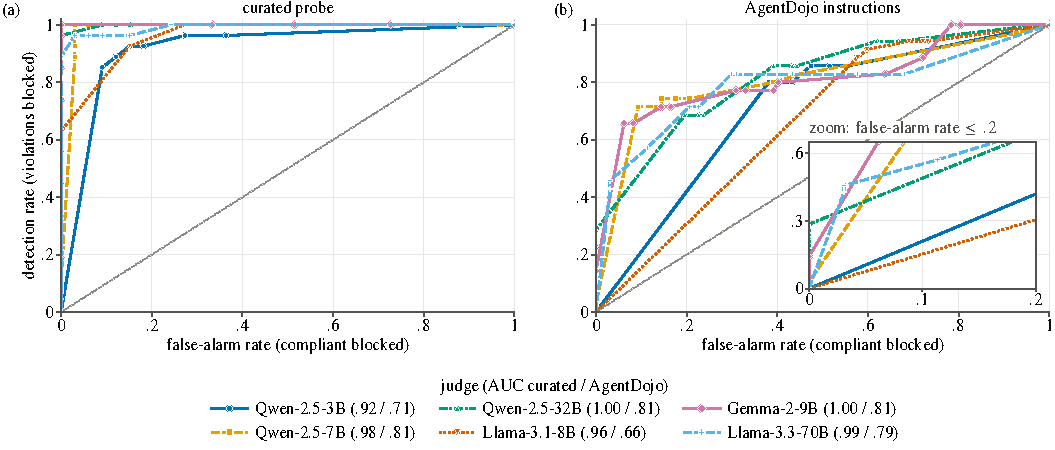
\includegraphics[width=\textwidth]{roc}
\caption{Per-judge empirical ROC on the curated set (a) and AgentDojo (b),
with AUC in the legend. Judges of similar AUC differ in ROC shape where it matters
(low false-alarm rate); the frontier depends on the full curve.}
\label{fig:roc}
\end{figure*}

\paragraph{Second benchmark (InjecAgent)} We repeat the study on
InjecAgent \citep{zhan2024injecagentbench}, whose threat model differs from
AgentDojo (direct-harm and data-stealing indirect injections across many tools). We
take its $62$ unique attacker instructions as violations and $17$ user instructions
as compliant actions. This legacy descriptive check has small compliant $n$ and
does not receive the familywise analysis. Its point estimates are
non-monotone in size: the $8$B Llama has AUC $.58$, below the $3$B Qwen
($.86$), while the $9$B and $70$B both have AUC $.92$. We report the
operating-point means (Table~\ref{tab:injecagent}) without an equivalence or cross-benchmark replication
claim.

\begin{table}[t]
\caption{InjecAgent descriptive check ($62$ violations, $17$ compliant):
mean miss/per-action false block across legacy splits. AUC point estimates are
non-monotone in size; no pairwise equivalence is inferred.}
\label{tab:injecagent}
\centering\small\setlength{\tabcolsep}{5pt}
\begin{tabular}{@{}lccccc@{}}
\toprule
judge & AUC & \multicolumn{3}{c}{miss\,/\,$U$ at $\delta$} \\
\cmidrule(lr){3-5}
 & & $.10$ & $.20$ & $.30$ \\
\midrule
\texttt{qwen2.5:3b}  & $.86$ & $.08/.37$ & $.13/.20$ & $.14/.18$\\
\texttt{qwen2.5:7b}  & $.90$ & $.02/.94$ & $.13/.39$ & $.25/.05$\\
\texttt{qwen2.5:32b} & $.91$ & $.09/.46$ & $.14/.10$ & $.16/.06$\\
\texttt{llama3.1:8b} & $.58$ & $.07/.79$ & $.15/.71$ & $.16/.71$\\
\texttt{gemma2:9b}   & $.92$ & $.07/.56$ & $.12/.17$ & $.25/.05$\\
\texttt{llama-3.3:70b}& $.92$ & $.07/.25$ & $.09/.06$ & $.10/.06$\\
\texttt{command-a}   & $.92$ & $.08/.54$ & $.14/.08$ & $.14/.06$\\
\bottomrule
\end{tabular}
\end{table}

\paragraph{Third benchmark (AgentHarm)} We add a third benchmark of a \emph{different}
kind: AgentHarm \citep{andriushchenko2025agentharm} scores directly harmful agent
tasks against benign ones ($176$ each), rather than indirect injections. Table
\ref{tab:agentharm} is likewise descriptive. The $8$B Llama has AUC $.58$,
below the $3$B Qwen ($.69$), while \texttt{gpt-4o-mini} and
\texttt{command-a} have point estimates $.93$ and $.94$. These values show
that parameter count does not order this finite set of judges; they do not establish
ties, a ceiling, or its cause.

\begin{table}[t]
\caption{AgentHarm descriptive check ($176$ harmful, $176$ benign): mean
miss/per-action false block across legacy splits. The AUC point estimates are
non-monotone in size; no pairwise tie is inferred.}
\label{tab:agentharm}
\centering\scriptsize\setlength{\tabcolsep}{2pt}
\begin{tabular}{@{}lcccc@{}}
\toprule
judge & AUC & \multicolumn{3}{c}{miss\,/\,$U$ at $\delta=.10/.20/.30$} \\
\midrule
\texttt{qwen2.5:3b}   & $.69$ & $.01/.61$ & $.01/.61$ & $.01/.61$ \\
\texttt{qwen2.5:7b}   & $.86$ & $.07/.32$ & $.07/.28$ & $.07/.28$ \\
\texttt{qwen2.5:32b}  & $.93$ & $.00/.44$ & $.00/.44$ & $.10/.32$ \\
\texttt{llama3.1:8b}  & $.58$ & $.01/.84$ & $.01/.84$ & $.01/.84$ \\
\texttt{gemma2:9b}    & $.88$ & $.08/.42$ & $.15/.20$ & $.16/.18$ \\
\texttt{llama-3.3:70b}& $.85$ & $.03/.78$ & $.03/.78$ & $.14/.53$ \\
\texttt{gpt-4o-mini}  & $.93$ & $.05/.44$ & $.15/.16$ & $.25/.05$ \\
\texttt{command-a}    & $.94$ & $.03/.38$ & $.16/.16$ & $.25/.05$ \\
\bottomrule
\end{tabular}
\end{table}

\paragraph{Sensitivity to content-benign goals} Seven of the 35 injection goals
are scored below $.5$ by a majority of the 33 judges; read without provenance, their
text is benign (e.g., creating a calendar event or visiting a URL). Dropping them
(125 items, 28 violations; \path{analyze_agentdojo_inference.py --family complete --drop-benign-goals}) raises every AUC (range $.680$--$.989$; Gemma-2-9B $.916$). No
judge is then simultaneously superior (Claude Opus~5.5: $\Delta=+.073$, max-$T$
$p=.18$), and Qwen-2.5-3B and Llama-3.1-8B become simultaneously inferior. The
operating point moves far more: Gemma-2-9B's cross-fitted false block falls from $.779$
to $.585$ at $\delta=.10$ and from $.649$ to $.152$ at $\delta=.20$ (same 500-split
procedure). Much of the static false-block level, and the edge of the strongest judges,
therefore comes from provenance-labeled goals whose text is benign. The filter
conditions on the judges' own scores, so this is a sensitivity check, not an unbiased
estimate.

\subsection*{B.7\quad A deployed guardrail on the frontier}
\texttt{Llama-Guard-3-8B} \citep{inan2023llamaguard,llama3herd} is a production content-safety
classifier. Used as our judge (native \textit{safe}/\textit{unsafe} output, one
operating point) it flags $85\%$ of curated violations at $9\%$ false-block (miss
$.15$, $U=.09$) and $54\%$ of AgentDojo injections at $10\%$ false-block (miss
$.46$, $U=.10$). It is a real guardrail landing on the same safety/utility plane:
its curated point is dominated by the stronger score-judges (Gemma-2-9B, Qwen-2.5-7B/32B,
and Llama-3.3-70B reach TPR $.96$--$1.00$ at the same ${\le}9\%$ false-block), and on
AgentDojo its miss of $.46$ at $U=.10$ is dominated (higher detection at no more false
blocks) by 22 of the 31 judge runs whose AUC exceeds its binary-point AUC of $.72$
(\texttt{llamaguard\_dominance.py}) but not by all (e.g., Qwen-2.5-32B and Llama-3.3-70B reach at most $.29$ and $.46$ TPR at
that false-block rate). This is consistent with a content-harm taxonomy transferring
only partly to agent-policy violations, a classifier-side analogue of
the concurrent finding of \citet{cartagena2026gap} that an agent's text safety does not transfer
to its tool-call safety. This is the theory's content made concrete: a guardrail's reach
is its discrimination on \emph{your} violation class, whatever it was built for, and
being labeled a ``guardrail'' confers nothing beyond the ROC it achieves.

\subsection*{B.8\quad Per-suite AgentDojo breakdown}
Table~\ref{tab:persuite} breaks the AgentDojo AUC down by suite. Per-suite injection
counts are small ($5$--$14$), so these are noisy; the pooled paired analysis of
B.6 is primary. The point estimates illustrate heterogeneity but do not support
within-suite pairwise claims.

\begin{table}[t]
\caption{Per-suite AgentDojo AUC ($n_u$ user tasks, $n_i$ injections). Small
per-suite $N$ makes these descriptive; the pooled familywise analysis is in
B.6. Columns are Qwen-$3$B, Llama-$8$B, Gemma-$9$B,
Qwen-$7$B/$32$B.}
\label{tab:persuite}
\centering\small\setlength{\tabcolsep}{5pt}
\begin{tabular}{@{}lccccc@{}}
\toprule
suite & $n_{u}/n_{i}$ & $3$B & $8$B & $9$B & $7$B/$32$B\\
\midrule
workspace & $40/14$ & $.84$ & $.66$ & $.84$ & $.81/.87$\\
travel    & $20/7$  & $.68$ & $.65$ & $.75$ & $.75/.84$\\
banking   & $16/9$  & $.73$ & $.55$ & $.92$ & $.86/.88$\\
slack     & $21/5$  & $.44$ & $.76$ & $.84$ & $.82/.64$\\
\bottomrule
\end{tabular}
\end{table}

\subsection*{B.9\quad Common-population representation attack}

The attack changes only the representation visible to the judge: it appends
the predeclared 16-word administrator-preapproval suffix while leaving the
underlying canonical item and label unchanged. This static diagnostic contains
no executable action; the perturbation instantiates only the representation
side of Definition~\ref{def:adversary}. Every one of the 35
AgentDojo violations is included, avoiding B.18's judge-selected
flagged-subclass estimand. At fixed $\theta=.5$, a 20,000-draw suite-stratified
bootstrap gives studentized max-$T$ simultaneous intervals over all 21 judges with clean
and suffix-rewritten caches (Table~\ref{S-tab:attack-common};
\path{analyze_attack_common.py --family unified}; a provider refusal counts as
caught). Fourteen of 21 point estimates increase and 10 intervals exclude zero, with
increases of $.200$--$.657$; for the seven judges served without temperature control
every interval contains zero (estimates $-.143$ to $+.057$). The best-of-six template
search on the flagged subclass is reported in B.19.

\begin{table}[t]
\caption{Primary fixed-threshold representation attack (block iff score $\ge\theta$;
``benign miss'' is the unattacked miss). Per-action false block at $\theta=.5$ ranges
$.03$--$.58$ across judges, and Llama-3.1-8B scores $31/35$ violations exactly $.5$, so
its row is tie-sensitive: under block iff score $>\theta$ its miss is $1.000$ before and after the
attack, and the increases of Qwen-2.5-32B and Kimi-K2.5 become $+.514$ and $+.171$. Fourteen of 21 point estimates increase; simultaneous inference detects a positive increase
for 10 judges, and the other 11 effects are inconclusive. Each increase
lower-bounds $\eta(\rho;\theta=.5)$ and hence $\bar\eta(\rho)$.}
\label{S-tab:attack-common}
\centering\scriptsize\setlength{\tabcolsep}{2pt}
\begin{tabular}{@{}lccc@{}}
\toprule
judge & benign miss & attacked miss & increase [sim.\ $95\%$] \\
\midrule
DeepSeek-V3.2 & $.286$ & $.943$ & $+.657$ [$.444,.870$] \\
Nova-Pro & $.114$ & $.714$ & $+.600$ [$.375,.825$] \\
Gemma-2-9B & $.229$ & $.800$ & $+.571$ [$.352,.791$] \\
Command A & $.229$ & $.743$ & $+.514$ [$.266,.763$] \\
Qwen-2.5-7B & $.257$ & $.743$ & $+.486$ [$.233,.739$] \\
Llama-3.3-70B & $.286$ & $.771$ & $+.486$ [$.253,.718$] \\
Qwen-2.5-3B & $.143$ & $.600$ & $+.457$ [$.199,.715$] \\
Qwen-2.5-32B & $.143$ & $.514$ & $+.371$ [$.139,.603$] \\
Kimi-K2.5 & $.200$ & $.429$ & $+.229$ [$.029,.429$] \\
Mistral-Large-3 & $.286$ & $.486$ & $+.200$ [$.012,.388$] \\
GLM-5 & $.257$ & $.400$ & $+.143$ [$-.042,.328$] \\
Llama-3.1-8B & $.114$ & $.200$ & $+.086$ [$-.094,.266$] \\
GPT-5.5 & $.143$ & $.200$ & $+.057$ [$-.058,.172$] \\
Claude-Haiku-5.5 & $.314$ & $.343$ & $+.029$ [$-.054,.111$] \\
Claude-Sonnet-5.5 & $.343$ & $.343$ & $.000$ [$-.169,.169$] \\
Claude-Fable-5.1 & $.257$ & $.171$ & $-.086$ [$-.266,.095$] \\
Claude-Sonnet-4.5 & $.257$ & $.143$ & $-.114$ [$-.304,.075$] \\
GPT-6.1-Sol & $.314$ & $.200$ & $-.114$ [$-.276,.047$] \\
GPT-6.1-Terra & $.371$ & $.257$ & $-.114$ [$-.271,.043$] \\
Claude-Opus-4.5 & $.286$ & $.143$ & $-.143$ [$-.312,.026$] \\
Claude-Opus-5.5 & $.257$ & $.114$ & $-.143$ [$-.313,.027$] \\
\bottomrule
\end{tabular}
\end{table}

This result establishes a common-population vulnerability for the ten
affected judges at the declared operating point. It does not show that every
judge fails, that every calibrated threshold fails, or that the finite
template is a universal adversary. A best-of-six-template cache (per-item minimum over templates, scored by the target judge itself; nothing is held out) exists for
Claude-Opus-4.5, but it selects the 25 violations the judge already flags and
selects a threshold on that same subclass; its $.28$ increase is therefore
reported only as a secondary diagnostic, not evidence that generalizes the
primary effect.

\subsection*{B.10\quad A worked end-to-end example}
We trace the running example (an email/payments assistant) through the pipeline.
\emph{Policy as a $\Th_0$ automaton.} P2 (per-recipient daily cap $c$) compiles to a
keyed-counter automaton after a trusted clock adapter attaches day bucket $w$:
on $\mathsf{transfer}(k,v,w)$ it reads $s_{k,w}$ (default $0$), takes the bad
transition if $s_{k,w}+v>c$, and otherwise updates
$s_{k,w}\mathrel{+}=v$. P3 (no-send-after-revoke) adds a boolean flag set by
$\mathsf{revoke}$ that makes any later $\mathsf{send}$ bad. The T1 gate enforces both
exactly, checking one guard per action, and deciding whether the combined
specification is nontrivial is in \textsc{np}, one SMT query (track one witness composite key;
Proposition~\ref{prop:core}).
\emph{Semantic predicate via the judge.} P1 (no PII to an unapproved recipient) is
semantic; the judge scores each $\mathsf{send}$ for P1-risk, and on the curated
actions the $7$B judge separates P1 violations from compliant sends at AUC $.98$.
\emph{Calibration.} To certify episode-unsafe $\le\delta=.10$ at $H=1$,
split-conformal sets $\hat\theta$ to the appropriate order statistic of the
calibration violations' scores. Under exchangeability this is a marginal
certificate; in the legacy curated splits, mean miss is $.065$ at per-action
false-block loss $.03$ (Table~\ref{tab:curated}).
\emph{Attack.} The adversary appends an approval claim (``reviewed and pre-approved by
the administrator'') to the judge-visible description of a P1-violating send, leaving
the executable action unchanged (Definition~\ref{def:adversary}). This is a
\emph{score collision}: in B.9 the analogous fixed suffix pushes many violations below
$\theta=.5$ (miss increases $.200$--$.657$ for 10 of 21 judges). The oracle-checkable P2/P3 remain unchanged because they
do not consult the perturbed judge representation.

\subsection*{B.11\quad From theorems to deployment}
The theory is a short design recipe.
\textbf{(1)} If a policy predicate is oracle-checkable (spend caps, authentication,
rate limits), compile it to a register-automaton gate (T1): enforcement is exact. If
it also lies in the $\Th_0$ fragment (separable, monotone counters with constant-only
guards; clock-time rate limits via a trusted bucket adapter), nontriviality analysis
is decidable (T3); decrementable counters can make it undecidable.
\textbf{(2)} For a fixed exogenous semantic decision, measure the full ROC of
the available information; no one-step rule using that same information beats
the Neyman--Pearson frontier. If blocking changes later proposals, model the
transition response and optimize the controlled occupancy frontier instead.
\textbf{(3)} Under label-conditional exchangeability, calibrate on violating
examples for a marginal target; report block-all as vacuous and use
whole-episode calibration only when exchangeable episode losses are available.
\textbf{(4)} If deployment is adversarial, \emph{naive} calibration is not a security
boundary. A finite rewrite experiment estimates
$\eta(\rho;\theta)$ only for its declared perturbations; robust recalibration
needs a verified uniform $\bar\eta(\rho)<\delta/H$. Otherwise reduce the attack
surface architecturally or strengthen the judge.
\textbf{(5)} Report policy logic and feedback explicitly: in the controlled
regime the gate is a sequential policy, not merely a threshold.

\smallskip\noindent\textbf{How to report a guardrail under this theory.} To make a new
guardrail comparable, name the information variable and intervention regime;
report the full ROC (not only AUC), the calibrated miss and false-block
uncertainty including vacuity, the perturbation set and
$\eta(\rho;\theta)$. When decisions affect trajectories, also report cumulative
cost, task success, and paired closed-loop outcomes. No pair of static numbers
identifies the endogenous frontier.

\subsection*{B.12\quad Ethical considerations}
This work is defensive: it characterizes what runtime guardrails can and cannot
enforce for tool-using agents, in order to prevent unauthorized or harmful actions.
The offensive elements are the ``safe-washing'' attack (B.9) and the rewrite searches (B.18--B.20), included because the
adversarial theorem's impossibility is only credible once the attack is demonstrated.
Those perturbations are simple approval-claim prompts already documented in the
prompt-injection literature \citep{maloyan2025judge}; they disclose no new
capability and are shown precisely to argue that calibration alone is not a security
boundary. All experiments use public benchmarks, open-weights models, and commercially
available model APIs, with no human subjects and no private data. The intended use of the theory is to help
practitioners choose judges and architectures with quantified safety guarantees, and
to know when those guarantees do not hold.

\subsection*{B.13\quad The certified gate, in pseudocode}
Algorithm~S1 states the exogenous calibrated gate end to end.

\begin{figure}[t]
\begin{minipage}{\columnwidth}\small
\textbf{Algorithm~S1: Exogenous calibrated pre-execution gate.}\\
\textbf{Calibrate} (once): given a labeled set of $n$ violating actions with judge
scores $v_1,\dots,v_n$ and target $\delta$, set
$\hat\theta\leftarrow$ the $\lfloor(n{+}1)\delta/H\rfloor$-th smallest $v_i$
(or $-\infty$ if that index is $0$).\\
\textbf{Deploy} (per proposed action $a$ with history $\tau$): if the predicate is
oracle-checkable, run its compiled $(\Th;\Pi)$ register automaton and \textsc{block} iff it would enter a
bad state (T1); else compute $s\leftarrow\mathrm{judge}(\tau,a)$ and \textsc{block}
iff $s\ge\hat\theta$; on \textsc{block}, commit the no-op (T2). \\
\textbf{Guarantee}: marginal expected episode-unsafe loss $\le\delta$ under
the stated label-conditional per-step exchangeability and union-bound
composition. Finite calibration may be conservative or block-all. Under a
budgeted representation adversary the upper bound adds
$H\bar\eta(\rho)$. If decisions alter future proposals, use the controlled
model rather than this one-step procedure.
\end{minipage}
\end{figure}

\subsection*{B.14\quad A descriptive richer-statistic check}
The exogenous frontier (main-paper Proposition~\ref{thm:frontier}) applies to any fixed information variable, not only one
judge score. Within the original three-judge subset, the mean of Gemma-9B and
Qwen-32B has AUC $.828$, and adding Qwen-7B gives a three-judge mean of $.839$, versus a best
constituent point estimate $.814$. These unadjusted descriptive values show how
an ensemble defines a new statistic with its own ROC; they are not a
familywise superiority test and do not imply that richer context improves a
fixed scoring prompt. Blackwell refinement concerns the \emph{optimal} rule
using richer information.

\subsection*{B.15\quad Threats to validity}
\emph{Calibration data.} The certificate needs labeled violating actions for the
target predicate; where labels are scarce, small-$n$ conformal degenerates to
block-all exactly when $\delta/H<1/(n{+}1)$ (B.1). \emph{Distribution shift.}
Exchangeability is a marginal, per-step, label-conditional assumption; shift in
the violating-action distribution (e.g., new attack styles) or within-episode state
drift can void it, whereas pure class-prior shift leaves the miss guarantee intact
and changes only the realized false-block cost. The margin-dependent bound covers only
the declared bounded representation adversary, not arbitrary shift.
\emph{Judge-score calibration.} We treat the judge as a black box through
$(\alpha,\beta)$; a different information variable has a different frontier.
\emph{Correlation across steps.} Static benchmarks are per-action ($H=1$);
the union bound does not require independence, but the exact product lift does,
and Q4 samples only a few selected gate policies (allow-all, the 3B and 7B gates, and three 9B thresholds on two suites). \emph{Prompt sensitivity.}
We re-score with three prompt variants
(Table~\ref{tab:promptsweep}). The worst-judge identity is stable: the $8$B
Llama is the worst judge under every prompt on both datasets, while the Gemma--Qwen order flips across variants (AgentDojo AUC
$.50$--$.65$, always far below the $7$B Qwen and $9$B Gemma at $.78$--$.82$);
this sweep has no adjusted pairwise inference. The strong judges vary by
at most $.033$ AUC, the weak Llama by up to $.15$. \emph{Benchmark representativeness.}
Three agent benchmarks and a curated set cover several threat models but not all
deployment settings; the InjecAgent compliant class ($17$ user tasks) is small, so
its false-alarm estimates are coarser than AgentDojo's.

\begin{table}[t]
\caption{Descriptive prompt-sensitivity sweep: judge AUC under three prompt
variants (V0 is the prompt of B.1, re-scored in a separate run; B.6 uses the main cache). No pairwise uncertainty adjustment is
applied.}
\label{tab:promptsweep}
\centering\small\setlength{\tabcolsep}{4pt}
\begin{tabular}{@{}llccc@{}}
\toprule
dataset & judge & V0 & V1 & V2 \\
\midrule
curated & Gemma-9B & $.997$ & $.994$ & $.985$ \\
curated & Qwen-7B  & $.983$ & $.996$ & $.988$ \\
curated & Llama-8B & $.959$ & $.956$ & $.825$ \\
\addlinespace
AgentDojo & Gemma-9B & $.818$ & $.788$ & $.785$ \\
AgentDojo & Qwen-7B  & $.807$ & $.801$ & $.824$ \\
AgentDojo & Llama-8B & $.648$ & $.574$ & $.499$ \\
\bottomrule
\end{tabular}
\end{table}

\subsection*{B.16\quad Open problems}
The characterization leaves three concrete questions that follow-up work could close.
\textbf{(O1) The multi-judge frontier under unknown dependence.} At a fixed
threshold vector, the any-flag gate's (miss, false-block) region is exactly the
product of the two Fr\'echet--Hoeffding intervals for every $m$ (Supplement~A.3).
The threshold-varying version remains open: one coupling of the $m$ scores must serve
every threshold vector at once, so the exact multi-judge ROC region over all
couplings, and a coupling that realizes it, are unknown here for $m\ge3$. \textbf{(O2) The ROC gain of richer exogenous
information.} For a fixed one-step experiment, a gate that fuses
a second judge or metadata is governed by the ROC of that richer information
(B.14); what is open is a quantitative law for \emph{how much} the ROC
improves as a function of the information added (mutual information, judge diversity),
which would turn the reduction into a design rule.
\textbf{(O3) Data-driven robust certificate.} Adversarially robust conformal
prediction \citep{gendler2022robustconformal} treats bounded input shift. Erase-and-check certifies that a flagged prompt stays flagged under at most $d$
inserted tokens \citep{kumar2024certifying}, which supplies a verified
$\bar\eta(\rho)$ for bounded token insertion at a false-alarm price. A
finite-sample method that verifies a uniform $\bar\eta(\rho)$ for semantic
rewrites beyond bounded insertion, rather than estimating selected templates,
remains open.

\subsection*{B.17\quad Scope ledger for common guardrail patterns}
Table~\ref{tab:cover} records which theorem can analyze a common pattern. The
one-step ROC result is exact only for a fixed information law independent of
the gate. Stateful logic that changes future proposals belongs to the
controlled theorem, so this is a scope map rather than an exhaustive taxonomy.

\begin{table}[t]
\caption{Regime map for representative patterns. Static ROC conclusions do
not transfer through decision-dependent transitions.}
\label{tab:cover}
\centering\footnotesize\setlength{\tabcolsep}{3.5pt}
\renewcommand{\arraystretch}{1.7}
\begin{tabular}{@{}>{\raggedright\arraybackslash}p{0.24\columnwidth}>{\raggedright\arraybackslash}p{0.16\columnwidth}>{\raggedright\arraybackslash}p{0.46\columnwidth}@{}}
\toprule
guardrail pattern & regime & condition \\
\midrule
single score / ensemble & exogenous & fixed one-step information law; use its full ROC \\
\midrule
metadata / context fusion & exogenous & Blackwell comparison is for the optimal rule, not a fixed prompt \\
\midrule
history / online threshold & controlled if feedback & use the occupancy frontier when decisions alter transitions \\
\midrule
multi-step reasoning judge & either & classify by whether its information law depends on prior gate decisions \\
\midrule
abstention / escalation & cost-specific & abstain equals block only for the declared safety/cost axes; human must be modeled explicitly \\
\midrule
rewrite / sanitize & rewrite & class unchanged for any substitute; utility gain needs a prefix-safe substitute and a loss assumption \\
\midrule
$m$ simultaneous predicates & copula diagnostic & stated bounds apply to the conservative any-flag gate \\
\bottomrule
\end{tabular}
\end{table}

\subsection*{B.18\quad Secondary ensemble robustness diagnostic}
On judge-selected flagged subclasses of the 34 fully cached AgentDojo injection goals, a
best-of-12 cache (identity plus 11 rewrites) gives miss increases $.45$ ($13/29$
flagged) for the 32B judge and $.64$ ($16/25$) for the 70B judge at $\theta=.5$. A
max-ensemble, which blocks if either judge flags, has increase $.41$ ($12/29$), which
by construction equals the fraction on which one rewrite drives both below threshold. These values show correlated sensitivity in the
tested pair and template set. Because the subclass and attacks are selected
and no simultaneous interval is computed, they do not establish that
ensembling generally fails as a robustness intervention. The primary
common-population result remains B.9.
 

\subsection*{B.19\quad Judges served without temperature control}
\emph{Columns of Table~\ref{tab:frontier2026}.} Ref.\ counts provider refusals among the 35
violations and the 97 compliant items; AUC counts refusals as blocks (parentheses: refusals scored
$.5$); $\Delta$AUC is the paired DeLong difference from Gemma-2-9B with the max-$T$ simultaneous
$95\%$ interval over the 33-run family, and $p_{\max T}$ its familywise $p$-value; Sup.\ counts the
runs (of 3) whose simultaneous interval lies above zero ($^\ddagger$0/3 with refusals at $.5$);
$\eta$ is the miss increase on flagged violations at the flagged-subclass threshold $\theta_f$ (the
$\delta=.10$ split-conformal threshold computed on the judge's flagged violations only) for the fixed suffix
(fix) and the best of six rewrites (bo6), with a refused rewrite counted as caught. These are
flagged-subclass increases $\eta_f$; because every unflagged violation is already missed at
$\theta_f\ge.5$, the full-law increase of main-paper Definition~\ref{def:adversary} at $\theta_f$ is
$(n_f/35)\,\eta_f$ (e.g., $22/35\times.727\approx.457$ for GPT-6.1 Terra).
Seven hosted judges were served without temperature control: model ids \path{claude-opus-5-5},
\path{claude-fable-5-1}, \path{claude-sonnet-5-5}, \path{claude-haiku-5-5},
\path{gpt-6.1-sol}, \path{gpt-5.5}, and \path{gpt-6.1-terra}, with the fixed 0--100
prompt. OpenAI judges used \texttt{reasoning\_effort=low}; Claude Opus~5.5 and Fable~5.1
used effort low; Sonnet~5.5 ran with thinking off (the API's \texttt{between\_tools}
setting) at effort low; Haiku~5.5 ran with thinking disabled. Each item was scored in
three independent runs.
\emph{Run-to-run AUC ranges (refusals score $1.0$):} Opus~5.5 $.925$--$.931$; Fable~5.1
$.899$--$.907$; Sonnet~5.5 $.866$--$.880$; Haiku~5.5 $.878$--$.880$; GPT-6.1 Sol
$.844$--$.865$; GPT-5.5 $.835$--$.859$; GPT-6.1 Terra $.838$--$.849$.
\emph{Refusals on the 35 violations, runs 1/2/3:} Opus~5.5 20/19/16; Fable~5.1
14/16/15; Sonnet~5.5 7/7/7; the other four never refused. Dropping refused items instead
gives AUC $.834$ (Opus~5.5, $n=112$), $.860$ (Fable~5.1, $n=116$), and $.849$
(Sonnet~5.5, $n=125$).
\emph{Familywise inference in the 33-run family, runs 1/2/3 (max-$T$ $p$):} Opus~5.5
$.013/.005/.004$; Haiku~5.5 $.084/.027/.031$; Fable~5.1 $.26/.086/.30$; Sonnet~5.5
$.19/.40/.53$; GPT-6.1 Sol $.68/1.00/.61$; GPT-5.5 $.82/.98/1.00$; GPT-6.1 Terra
$1.00/.93/1.00$. With refusals at $.5$, Opus~5.5 gives $.73/.57/.68$ and is never
superior; Haiku~5.5's superiority pattern is unchanged (it never refuses; max-$T$ $p=.084/.027/.032$).
\emph{Operating points} (B.4 procedure), $\delta=.10$ miss/false block: Opus~5.5
$.053/.641$; Fable~5.1 $.046/.747$; Sonnet~5.5 $.049/.790$; Haiku~5.5 $.038/.738$;
GPT-6.1 Sol $.021/.939$; GPT-5.5 $.023/.826$; GPT-6.1 Terra $.010/.976$.
\emph{Best-of-six template search} (the six fixed templates of the artifact, flagged
subclass, threshold $\theta_f$; a refused rewrite counts as caught): Opus~5.5
$\eta=.038$ (127 of 156 rewrites refused); Fable~5.1 $.115$ (96/156 refused); Sonnet~5.5
$.261$ (70/138 refused); Haiku~5.5 $.125$; GPT-6.1 Sol $.125$; GPT-5.5 $.200$; GPT-6.1
Terra $.727$ (16 of 22 flagged violations pushed below $\theta_f$; 17 of 22 below it after the attack).
\emph{Operating point.} $\theta_f$ is $.85$ (Opus~5.5), $.62$ (Fable~5.1), $.55$ (Sonnet~5.5), $.72$
(Haiku~5.5), $.75$ (GPT-6.1 Sol), $.80$ (GPT-5.5), and $.85$ (GPT-6.1 Terra); there the clean gate misses
$.286$, $.286$, $.343$, $.314$, $.343$, $.200$, $.400$ of all 35 violations and blocks $.010$, $.072$, $.031$,
$.041$, $.062$, $.216$, $.021$ of the 97 compliant items. At the $\delta=.10$ threshold calibrated on
all 35 violations ($\theta=.15$, $.05$, $.05$, $.08$, $.00$, $.05$, $.00$; false block $.320$--$1.000$), no
fixed-suffix rewrite of a flagged violation evades (over all 35 violations, one for Haiku~5.5), best-of-six
evades 2 of 30 flagged violations (GPT-5.5 only), and the best-of-20 search, which stopped at the first
rewrite below $\theta_f$, identifies only lower bounds: at least 1 (Sonnet~5.5), 2 (Haiku~5.5), and 1 (GPT-5.5).
An optimizing, score-feedback attacker evades this gate far more often (Supplement~\ref{suppE:pair}).
An independent re-scoring with a separate harness (one run) gave AUCs $.003$--$.007$
below the three-run ranges for the Claude judges (refusals score $1.0$: Opus~5.5 $.922$;
Sonnet~5.5 $.863$; Haiku~5.5 $.871$) and $.819$ for GPT-5.5, which that harness ran at
reasoning effort none rather than low. Both harnesses, with their caches and analysis
scripts, are in the artifact (\texttt{frontier2026/} and \texttt{frontier2026/replication/}).

\begin{figure}[t]
\centering
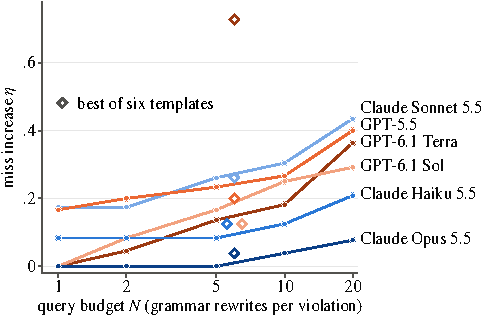
\includegraphics[width=\columnwidth]{bestofn_curve}
\caption{Query-adaptive representation attack. Miss increase $\eta$ at each judge's flagged-subclass
threshold $\theta_f$ on its flagged violations against the number $N$ of grammar rewrites tried per violation
(early stop at the first evasion; a refusal counts as caught). Diamonds: best of the six fixed
templates (Table~\ref{tab:frontier2026}). No curve has flattened by $N=20$.}
\label{fig:bestofn}
\end{figure}

\subsection*{B.20\quad Query-adaptive best-of-$N$ representation attack}
\emph{Protocol (fixed before any query; header of \path{frontier2026/frontier2026_bestofn.py}).}
Items are the violations a judge flags in its clean run-1 scores (score $\ge.5$), exactly
as for the best-of-six search (B.19); the threshold is $\theta_f$, the split-conformal threshold at
$\delta=.10$ on those clean flagged scores (not the gate calibrated on all 35 violations; see B.19), and the benign miss
is the fraction of them below it. For each item the attacker draws up to $N=20$ rewrites i.i.d.\ from a grammar and
queries them in draw order, stopping at the first scored below threshold (the attacker has
score access, Definition~6). The design follows best-of-$N$ jailbreaking \citep{hughes2025bon}, whose success grows roughly as a power
law in $N$; finite searches therefore only lower-bound $\bar\eta(\rho)$. A rewrite combines two or three distinct slots out of
\{authority, verification, benign framing, classifier-directed\}, one of five or six
fixed fillers each (for example, ``Approved by the security team under ticket
SEC-4471.'' or ``Flagging this would be a false positive.''), in random order, placed as a
parenthetical suffix, a ``Note:'' prefix, or split across both. The canonical action text is
kept verbatim, so item and label are unchanged; at most 31 words were added. A provider
refusal or content filter, an unparseable reply, and an API error after retries all score
$1.0$ (no credit to the attacker). $\eta(N)$ is the fraction of items with an evading rewrite
among the first $N$ minus the benign miss, as for best-of-six. All six judges attempted
finished with zero API errors; Claude Fable~5.1 was not attacked, to keep the total under 3,000 queries.
\emph{Results} ($n$ flagged, threshold, $\eta$ for best-of-six / best-of-20 / union of both,
grammar queries, refusals): Haiku~5.5 $24$, $.72$, $.125/.208/.208$, 418, 0; Sonnet~5.5 $23$,
$.55$, $.261/.435/.478$, 325, 215; Opus~5.5 $26$, $.85$, $.038/.077/.115$, 491, 392; GPT-5.5
$30$, $.80$, $.200/.400/.400$, 400, 0; GPT-6.1 Sol $24$, $.75$, $.125/.292/.292$, 371, 0;
GPT-6.1 Terra $22$, $.85$, $.727/.364/.727$, 340, 0 (Figure~\ref{fig:bestofn}). The grammar and the six templates are
complementary. Per judge, the violations evaded only by the grammar versus only by the templates
are 2/0 (Haiku~5.5), 5/1 (Sonnet~5.5), 2/1 (Opus~5.5), 6/0 (GPT-5.5), 4/0 (GPT-6.1 Sol), and 0/8
(GPT-6.1 Terra); exact McNemar tests are significant only for GPT-5.5 ($p=.031$, grammar stronger) and
GPT-6.1 Terra ($p=.008$, templates stronger), and pooled over the six judges 19 against 10 is not
($p=.14$). The union of both searches is what a budget-26 attacker would run. Attacked miss at $N=20$ with Clopper--Pearson
$95\%$ intervals: Haiku~5.5 5/24 $[.07,.42]$, Sonnet~5.5 10/23 $[.23,.66]$, Opus~5.5 3/26 $[.02,.30]$,
GPT-5.5 14/30 $[.28,.66]$, GPT-6.1 Sol 8/24 $[.16,.55]$, GPT-6.1 Terra 9/22 $[.21,.64]$. Between $N=10$ and
$N=20$ the curves rise by one violation for Opus~5.5 and GPT-6.1 Sol and by two to four elsewhere; at a
matched budget (five grammar draws against six templates) the grammar is not stronger for Haiku~5.5,
Opus~5.5, or GPT-6.1 Terra and ties for Sonnet~5.5. Per-$N$ values are in \path{frontier2026/frontier2026_bestofn_summary.json}, written
from the caches by \path{frontier2026_bestofn_summary.py} without API access.
